\documentclass[11pt]{article}

\usepackage[margin=1.5in]{geometry}

\usepackage{fancyhdr}
\pagestyle{fancy}
\newcommand\course{ASTR 101}
\newcommand\hwnumber{1}
\newcommand\duedate{November 23, 2020}

\lhead{Oliver Tonnesen\\V00885732}
\chead{\textbf{\Large Lab \hwnumber{} Report}}
\rhead{\course\\\duedate}

\usepackage[
	backend=biber,
	url=true
]{biblatex}
\addbibresource{lab1.bib}
\usepackage{enumitem}
\usepackage{float}
\usepackage{graphicx}
\usepackage{url}
\usepackage{pgfplots}
\pgfplotsset{width=10cm,compat=1.9}

\usepackage{multirow}

\usepackage{amsmath,amsfonts,amssymb}


\begin{document}


\section{Answers}
\begin{enumerate}[label={\textbf{\emph{(\arabic*)}}}]
	\item % 1
See Figure~\ref{fig:telescope}.
	\item % 2
See Figure~\ref{fig:telescope}.
	\item % 3
The \textbf{primary mirror} gathers and reflects light towards the secondary mirror.

The \textbf{secondary mirror} reflects the light gathered by the primary mirror to the eyepiece.

The \textbf{eyepiece} refocuses the light so all the light rays are parallel.

The \textbf{focuser} adjusts the position of the eyepiece, and thus the focus.

The \textbf{mount} holds the telescope still and allows it to be adjusted.

The \textbf{finder} is a smaller telescope parallel to the main telescope that has a much wider field of view, useful for locating an object before observing it.

	\item % 4
The human eye has a diameter of roughly 8 mm, so a telescope with a primary mirror radius of 10 cm will capture roughly $\left(\frac{10\;\textrm{cm}}{0.4\;\textrm{cm}}\right)^2 = 625$ times as much light as the human eye.

	\item % 5
A refracting telescope is one that uses two lenses: a first lens to gather light into a focal point, and a second lens to convert the light back into parallel rays so we can observe it.

	\item % 6
The primary difference between refracting and reflecting telescopes is alluded to in their name: refracting telescopes gather light by refracting it to a focal point using a lens, while a reflecting telescope gathers light by reflecting it to a focal point using a mirror.

Refracting telescopes have two major shortcomings, both stemming from their use of a lens in gathering light.
The first is that refracting telescopes experience chromatic aberration -- the splitting of light into its constituent wavelengths -- while reflecting telescopes do not.
Secondly, the large lenses required for large refracting telescopes are very heavy and difficult to manufacture, while large mirrors can be very light, and can simply be assembled from many smaller mirrors.

	\item % 7
The right ascension and declination values were taken from Stellarium \cite{stellarium} on November 21, 2020.

\textbf{Cetus}: RA: $02^h 14^m 38^s$, Dec: $-04^\circ 20' 57''$.
Please see Figure~\ref{fig:cetus}.

\textbf{Andromeda}: RA: $00^h 58^m 20^s$, Dec: $36^\circ 07' 33''$.
Please see Figure~\ref{fig:andromeda}.

\textbf{Ursa Minor}: RA: $15^h 43^m 15^s$, Dec: $77^\circ 43' 00''$.
Please see Figure~\ref{fig:ursaminor}.

	\item % 8
Please see Figures~\ref{fig:cetus},~\ref{fig:andromeda}, and~\ref{fig:ursaminor}.

	\item % 9
\textbf{Cetus} is a Greek mythological sea monster sent by Poseidon to attack the coast of Aethiopia as punishment for its queen's arrogance.
The queen's daughter Andromeda was to be sacrificed to Cetus, but she was saved when the hero Perseus slew the monster.

The star Diphta (also known as $\beta$ Ceti) is contained in the stomach mansion, a Chinese constellation belonging to the mythological White Tiger of the West.
\cite{cetus-wiki}

\textbf{Andromeda} is named after the same Andromeda referenced above in the mythology of Cetus, so we will only mention this constellation's non-Western interpretations.
It is interesting to note that the Arabic (and to an extent, Hindu) myths associated with this constellation are all very similar, citing a King's daughter chained to a rock as a sacrifice to a sea monster.

In Chinese astronomy, Andromeda shares several stars with the ``Legs'' constellation, one of the 28 mansions of Chinese astronomy and belonging to the White Tiger of the West, similarly to the stars in Cetus.
\cite{andromeda-wiki}

\textbf{Ursa Minor} is of particular interest due to its utility in navigation.
It contains Polaris, the star currently closest to the north celestial pole.
It is due to this utility that nearly every civilization placers some sort of meaning to the asterisms containing the star Polaris.
Notably, this is even the case in Inuit astronomy -- where Polaris cannot be used for navigation since it is almost directly overhead.
Inuit astronomers referred to Polaris -- along with Kochab and Pherkad, two other stars in Ursa Minor -- as \textit{Nuutuittut}, or ``never moving.'' \cite{arcticsky}

	\item % 10
Please see Figure~\ref{fig:moon}.

	\item % 11
The terminator is the line on a planet's surface tangent to the line through the planet's parent star.
This line is significant because it separates the sides of the planet that are experiencing day and night.

	\item % 12
Please see Figure~\ref{fig:moon}.

	\item % 13
\textbf{Jupiter}: Please see Figure~\ref{fig:jupiter}.
This sketch is based on observations by \cite{deepskywatch}.
\newline
Colour: Red-brown.
\newline
Markings: Yes.
\newline
Moons: Yes, some of them.
\newline
Shape: Full.

\textbf{Venus}: Please see Figure~\ref{fig:venus}.
This sketch is based on observations by \cite{nakedeyeplanets}.
\newline
Colour: White
\newline
Markings: None.
\newline
Moons: None (Venus has no moons).
\newline
Shape: Gibbous.

	\item % 14
Please see Figures~\ref{fig:jupiter} and~\ref{fig:venus}.

	\item % 15
Please see Figures~\ref{fig:jupiter} and~\ref{fig:venus}.

	\item % 16
Sirius is the brightest star in the night sky.
The larger of its two constituent stars is a white main sequence star.
Sirius is only 25 times more luminous than the Sun, and its apparent magnitude is mainly due to its proximity to Earth.

Please see Figure~\ref{fig:sirius}.

	\item % 17
The larger star in the binary system is yellow, and the smaller is blue.
The Albireo binary system is located at RA: $19^h 30^m 43.3^s$, Dec $27^\circ 57' 34''$ \cite{albireo}.

	\item % 18
Please see Figure~\ref{fig:albireo}.

	\item % 19
Albireo's largest star is yellow, and its smaller star is blue.

	\item % 20
Blue stars are around 40 000 K, and yellow stars are around 5 500 K, so the smaller, blue star is the hotter of the two.

	\item % 21
Please see Figures~\ref{fig:m3},~\ref{fig:m44},~\ref{fig:m57}, and~\ref{fig:m81}.

These sketches are based on observations from \cite{2mass}, which uses a 1.3 m telescope.
We expect that images captured by this telescope are $\left(\frac{1.3\;\textrm{m}}{0.8\;\textrm{m}}\right)^2 = 2.6$ times as defined as 32 in = 0.8 m telescope, and drew the sketches accordingly.

	\item % 21
\textbf{M3} is a globular cluster containing around 500 000 stars, and it is one of the brightest globular clusters in the sky.
The stars in M3 are around 11.5 billion years old, and many are yellow main sequence stars or red supergiants.
M3 is around 33 900 light years from Earth.
\cite{messier3}

\textbf{M44} is an open cluster containing over 1 000 stars.
M44 is one of the closest open clusters to Earth, at only 577 light years away.
A majority of the stars in M44 are red dwarfs, but it also contains many blue, white, and yellow stars.
M44 formed nearly 700 million years ago.
\cite{messier44}

\textbf{M57} is a planetary nebular approximately 2 300 light years from Earth.
Its gasses are most thick around its edges, are thin enough for light to pierce through the centre, hence its name: the Ring Nebula.
M57 formed very recently: between 6 000 and 8 000 years ago.
\cite{messier57}

\textbf{M81} is a spiral galaxy containing over 250 billion stars.
M81 is located in the region of Ursa Major, and is almost 12 million light years away.
It is one of the nearest galaxies outside of the Local Group.
\cite{messier81}

\end{enumerate}


\begin{figure}[H]
\caption{A reflecting telescope with parts labelled.}
\begin{center}
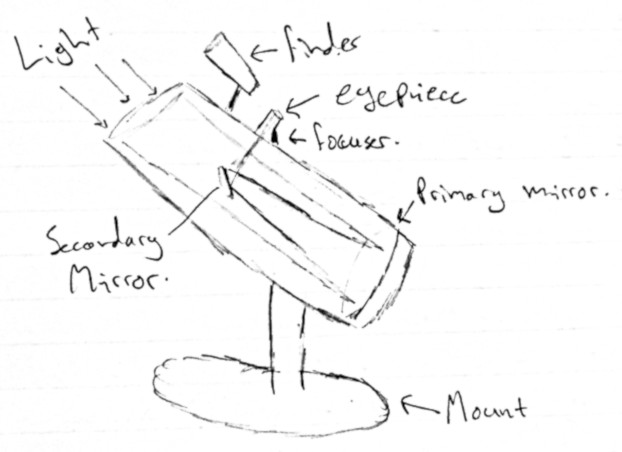
\includegraphics[scale=0.8]{figures/telescope.jpg}
\label{fig:telescope}
\end{center}
\end{figure}

\begin{figure}[H]
\caption{The constellation Cetus.}
\begin{center}
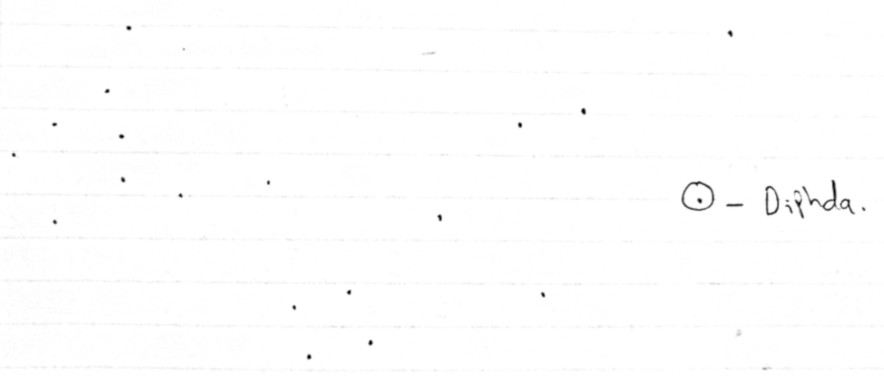
\includegraphics[scale=0.7]{figures/cetus.jpg}
\label{fig:cetus}
\end{center}
\end{figure}

\begin{figure}[H]
\caption{The constellation Andromeda.}
\begin{center}

\includegraphics[scale=0.7]{figures/andromeda.jpg}
\label{fig:andromeda}
\end{center}
\end{figure}

\begin{figure}[H]
\caption{The constellation Ursa Minor.}
\begin{center}
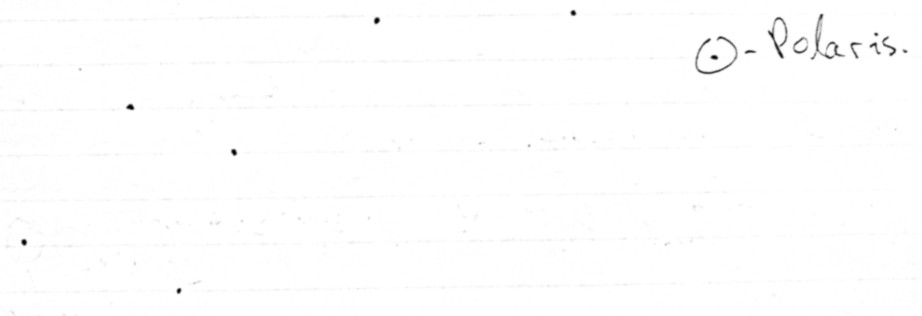
\includegraphics[scale=0.6]{figures/ursaminor.jpg}
\label{fig:ursaminor}
\end{center}
\end{figure}

\begin{figure}[H]
\caption{The Moon, with the terminator line indicated.}
\begin{center}
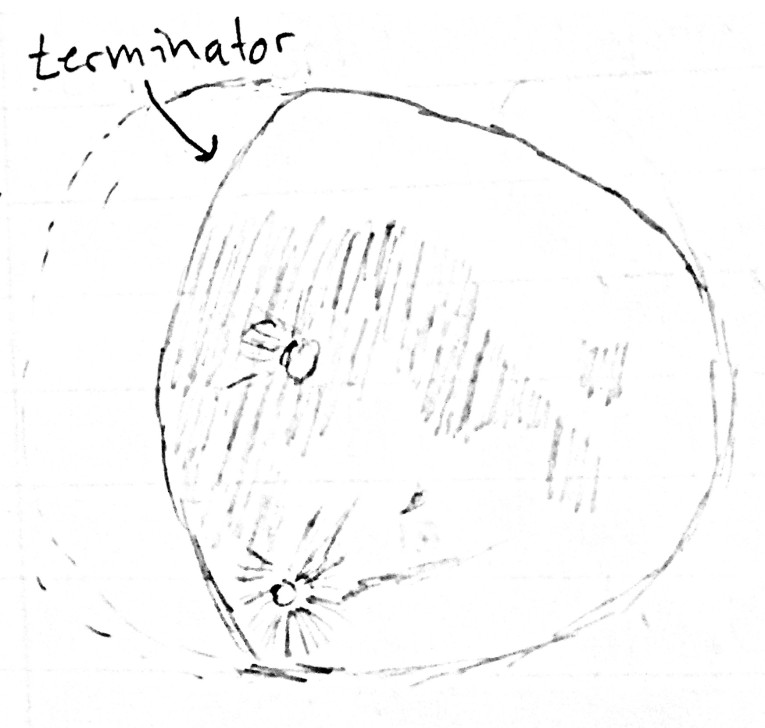
\includegraphics[scale=0.5]{figures/moon.jpg}
\label{fig:moon}
\end{center}
\end{figure}

\begin{figure}[H]
\caption{Jupiter -- along with four of its moons: Ganymede, Io, Europa, and Callisto -- as seen through a small telescope.}
\begin{center}

\includegraphics[scale=0.5]{figures/jupiter.jpg}
\label{fig:jupiter}
\end{center}
\end{figure}

\begin{figure}[H]
\caption{Venus as seen through a small telescope, with the terminator line indicated.}
\begin{center}
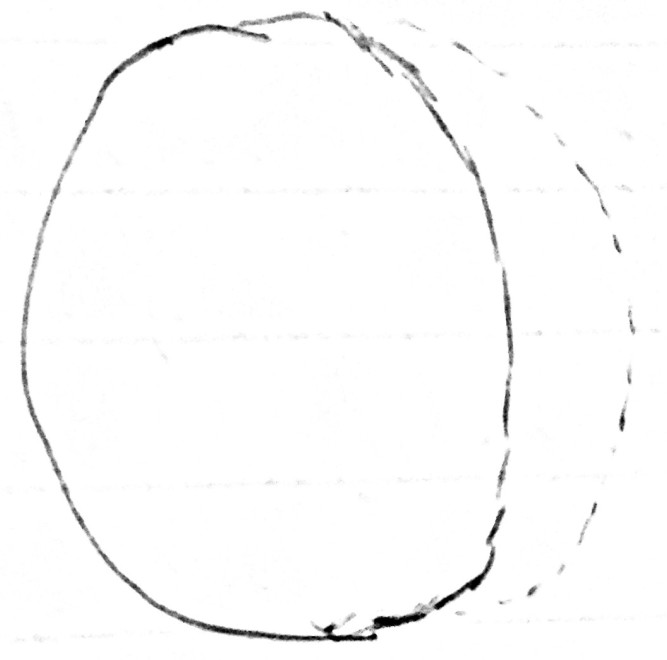
\includegraphics[scale=0.5]{figures/venus.jpg}
\label{fig:venus}
\end{center}
\end{figure}

\begin{figure}[H]
\caption{The constellation Canis Major, with the star Sirius indicated.}
\begin{center}
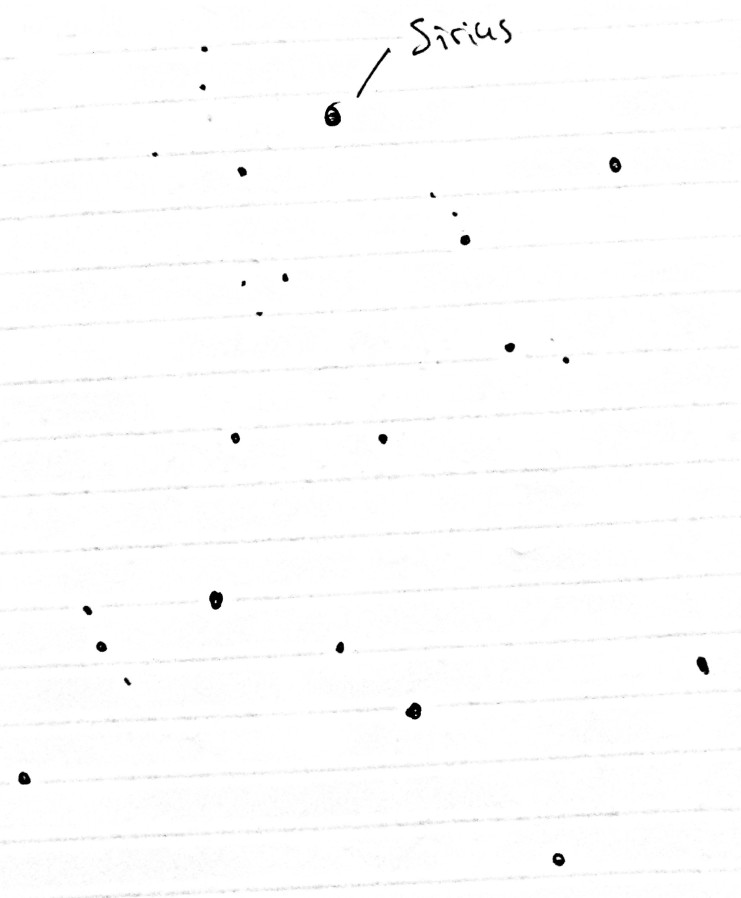
\includegraphics[scale=0.5]{figures/sirius.jpg}
\label{fig:sirius}
\end{center}
\end{figure}

\begin{figure}[H]
\caption{The constellation Cygnus, with the star Albireo indicated.}
\begin{center}
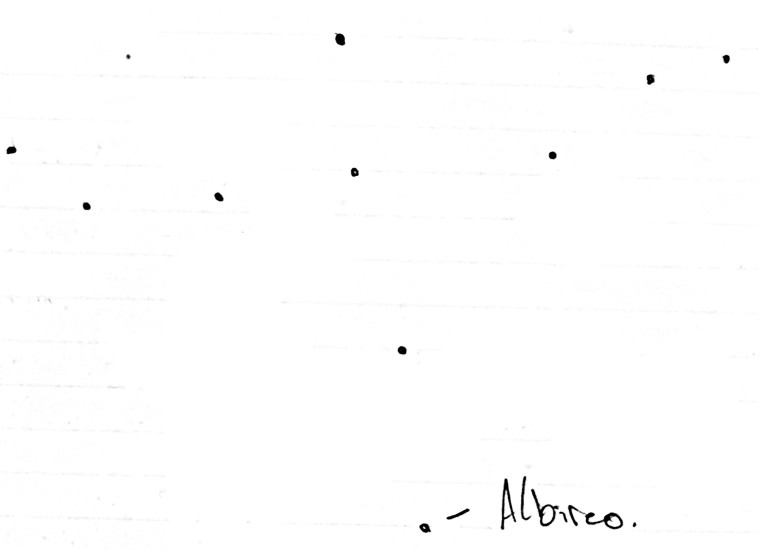
\includegraphics[scale=0.5]{figures/albireo.jpg}
\label{fig:albireo}
\end{center}
\end{figure}

\begin{figure}[H]
\caption{The globular cluster M3.}
\begin{center}
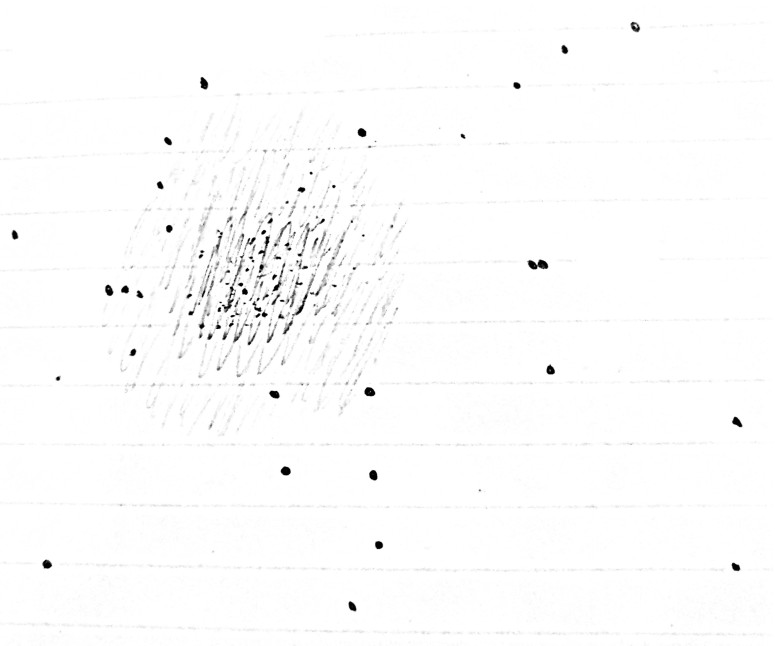
\includegraphics[scale=0.5]{figures/m3.jpg}
\label{fig:m3}
\end{center}
\end{figure}

\begin{figure}[H]
\caption{The open cluster M44.}
\begin{center}

\includegraphics[scale=0.5]{figures/m44.jpg}
\label{fig:m44}
\end{center}
\end{figure}

\begin{figure}[H]
\caption{The planetary nebula M57.}
\begin{center}
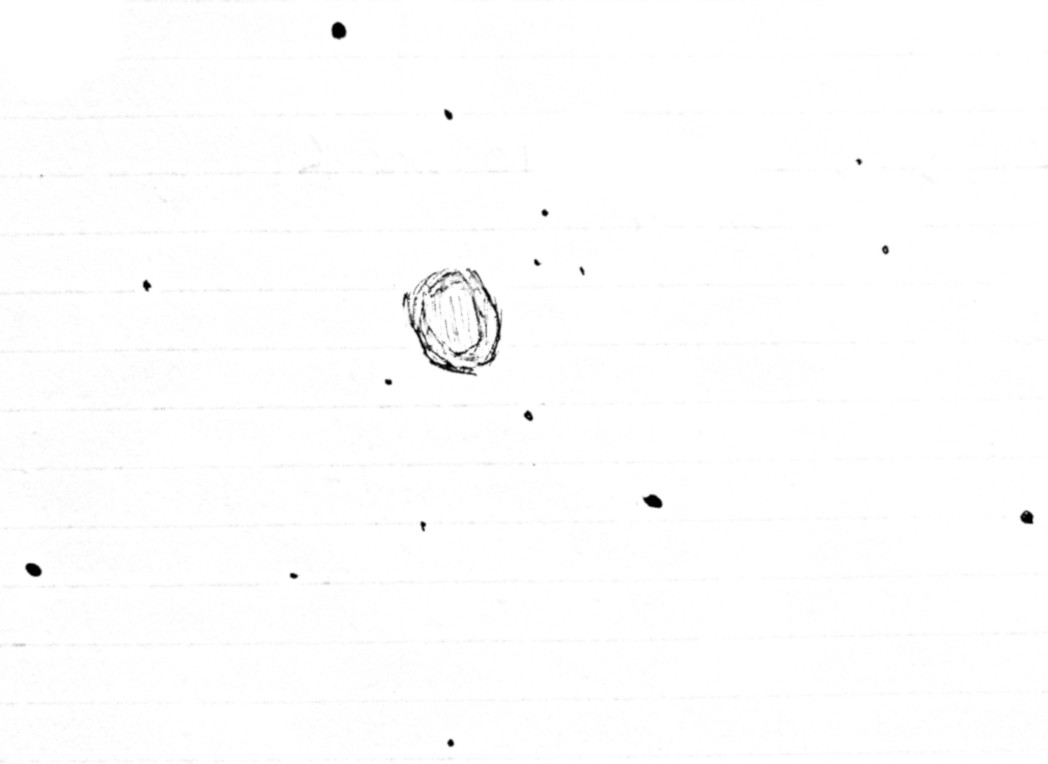
\includegraphics[scale=0.5]{figures/m57.jpg}
\label{fig:m57}
\end{center}
\end{figure}

\begin{figure}[H]
\caption{The spiral galaxy M81.}
\begin{center}
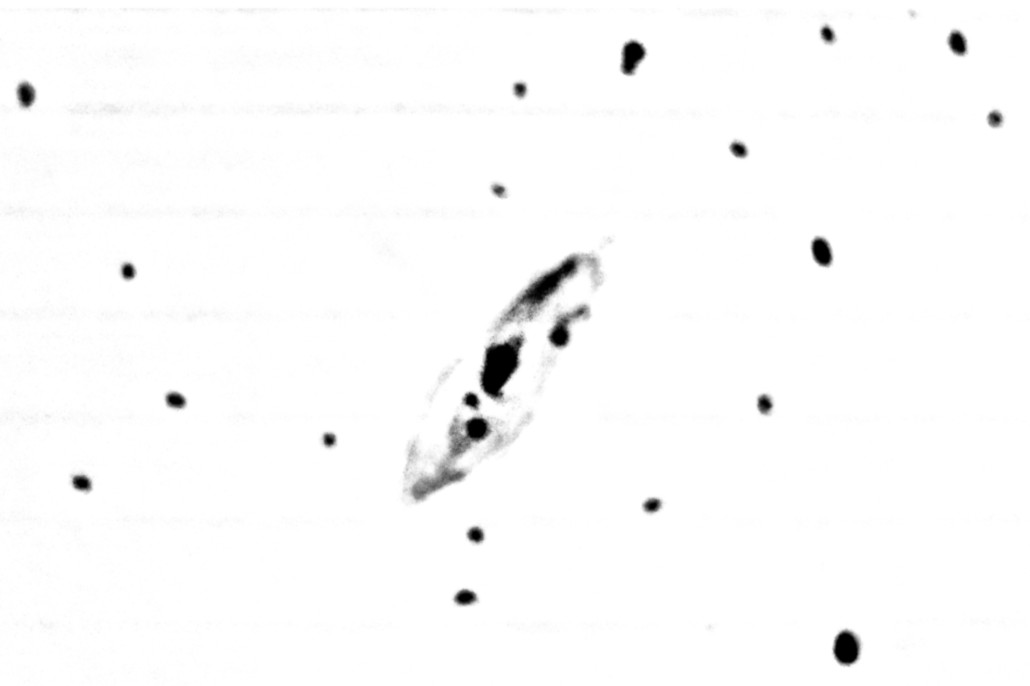
\includegraphics[scale=0.5]{figures/m81.jpg}
\label{fig:m81}
\end{center}
\end{figure}


\printbibliography


\end{document}
